%% LaTeX-Beamer template for KIT design
%% by Erik Burger, Christian Hammer
%% title picture by Klaus Krogmann
%%
%% version 2.1
%%
%% mostly compatible to KIT corporate design v2.0
%% http://intranet.kit.edu/gestaltungsrichtlinien.php
%%
%% Problems, bugs and comments to
%% burger@kit.edu

\documentclass[18pt]{beamer}
\usepackage[utf8]{inputenc} % for the umlauts

\beamertemplatenavigationsymbolsempty
%% SLIDE FORMAT

% use 'beamerthemekit' for standard 4:3 ratio
% for widescreen slides (16:9), use 'beamerthemekitwide'

\usepackage{templates/beamerthemekit}
% \usepackage{templates/beamerthemekitwide}

%% TITLE PICTURE

% if a custom picture is to be used on the title page, copy it into the 'logos'
% directory, in the line below, replace 'mypicture' with the 
% filename (without extension) and uncomment the following line
% (picture proportions: 63 : 20 for standard, 169 : 40 for wide
% *.eps format if you use latex+dvips+ps2pdf, 
% *.jpg/*.png/*.pdf if you use pdflatex)

%\titleimage{mypicture}

%% TikZ INTEGRATION

% use these packages for PCM symbols and UML classes
% \usepackage{templates/tikzkit}
% \usepackage{templates/tikzuml}

% the presentation starts here

\title[SWT1: Kurzvortrag]{Softwaretechnik 1 - Kurzvortrag}
\author{Felix Bachmann}

\institute{KIT - Institut für Programmstrukturen und Datenorganisation (IPD)}

% Bibliography

\usepackage[citestyle=authoryear,bibstyle=numeric,hyperref,backend=biber]{biblatex}
\addbibresource{templates/example.bib}
\bibhang1em

\begin{document}

% change the following line to "ngerman" for German style date and logos
\selectlanguage{ngerman}

%title page
\begin{frame}
\titlepage
\end{frame}

%table of contents
\begin{frame}{Themenübersicht}
\tableofcontents
\end{frame}

\section{Entwurfsmuster}
	\subsection{Was ist das?}
		\begin{frame}{Was ist das?}	
			\begin{block}{Definition aus der Vorlesung}
				Ein Software-Entwurfsmuster beschreibt eine Familie von Lösungen für ein Software-Entwurfsproblem.
			\end{block}
			\begin{itemize}
				\item Klassendiagramme, die bestimmte Probleme lösen/ einen Lösungsansatz geben
				\item das Rad nicht neu erfinden	
				\item erleichtern Kommunikation
				\item erleichtern "'gute"' Entwürfe und das Schreiben von wartbarem/erweiterbarem Code
			\end{itemize}
		\end{frame}

	\subsection{Kategorien}
		\begin{frame}{Kategorien}
			\begin{block}{Entkopplungs-Muster}
				\begin{itemize}
					\item mehrere unabhängige Einheiten kommunizieren durch Kopplungsglied untereinander
				\end{itemize}
			\end{block}
			\begin{block}{Varianten-Muster}
				\begin{itemize}
					\item Gemeinsamkeiten herausziehen, redundanter Code wird vermieden
				\end{itemize}
			\end{block}
			\begin{block}{Zustandshandhabungs-Muster}
				\begin{itemize}
					\item Bearbeitung des Zustands von Objekten (unabhängig vom Zweck)
				\end{itemize}
			\end{block}
			\begin{block}{Steuerungs-Muster}
				\begin{itemize}
					\item Steuerung des Kontrollflusses (richtige Methoden zur richtigen Zeit)
				\end{itemize}
			\end{block}
			\begin{block}{Bequemlichkeits-Muster}
				\begin{itemize}
					\item sparen Schreib- oder Denkarbeit
				\end{itemize}
			\end{block}
		\end{frame}

	\subsection{Beobachter/Observer}
		\begin{frame}{Beobachter/Observer: abstrakt}
			\begin{exampleblock}{Problemstellung}
				\begin{itemize}
					\item ein Subjekt, viele Beobachter
					\item Subjekt ändert Zustand $\implies$ Beobachter machen "'irgendwas"
				\end{itemize}		
			\end{exampleblock}
		\end{frame}
		
		\begin{frame}{}
			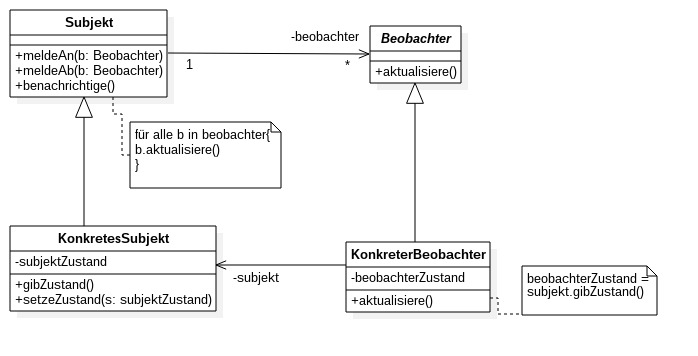
\includegraphics[keepaspectratio, width=\textwidth, height=\textheight]{diagrams/interview/observer.jpg}
			\pause
			\begin{block}{Vorteile des Entkopplungsmusters Beobachter}
				\begin{itemize}
					\item Beobachter definiert selber, was bei Benachrichtigung passiert, Subjekt kriegt davon nichts mit
					\item Subjekt kennt nur Interface der Beobachter, variable Anzahl Beobachter
				\end{itemize}
			\end{block}
		\end{frame}

		\begin{frame}{Beobachter/Observer: am Beispiel}
			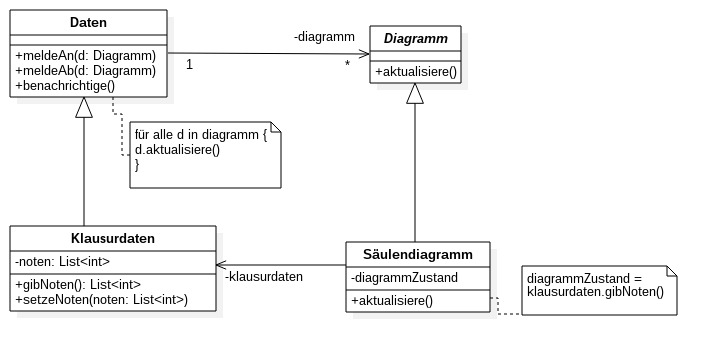
\includegraphics[keepaspectratio, width=\textwidth, height=\textheight]{diagrams/interview/observer_example.jpg}
			

\end{frame}

\end{document}
